\documentclass{article}
\usepackage[utf8]{inputenc}
\usepackage[american]{babel}
\usepackage[T1]{fontenc}
\usepackage{amssymb,amsthm,amsmath,amsfonts}
%\usepackage{algorithmic}
%\usepackage{algorithm}
\usepackage{tikz}
\usepackage{nicefrac}

\theoremstyle{plain}
\newtheorem{thm}{Theorem}
\newtheorem{lem}[thm]{Lemma}
\newtheorem{cor}[thm]{Corollary}
\newtheorem{prop}[thm]{Proposition}
\theoremstyle{definition}
\newtheorem{defi}[thm]{Definition}
\theoremstyle{remark}
\newtheorem{rem}[thm]{Remark}
\newtheorem{exe}[thm]{Example}

\author{Cyril Hugounenq}

\begin{document}

\section{Reminder on Couveignes' algorithm}


\section{Reminder on isogeny volcanoes}
\begin{defi}
Let $E$, $E'$ two elliptics curve such that there exists an isogeny $\phi: E \rightarrow E'$. If $E$ is separable then $deg(\phi)=ker(\phi)$. For $\ell$ an integer we call an $\ell$ isogeny, an isogeny of degree $\ell$
\end{defi}

\begin{defi}
A volcano of $\ell$ isogeny is a graph of $\ell$ isogenies of degree $\ell+1$.
\end{defi}

\begin{defi}
For $E$ an ordinary elliptic curve defined over $\mathbb{F}_q$ we denote  his endomorphism ring (associated up to isomorphism) by $\mathcal{O}$. $\mathcal{O}$ is an order include in a quadratic imaginary field denoted $K$, we denote $\mathcal{O}_K$ the algebraic integers of $K$.
\end{defi}

\begin{prop}
Let $E$ and $E'$ two elliptic curves defined over $\mathbb{F}_q$, $\phi :E \rightarrow E'$ an $\ell$-isogeny, with $\ell \neq p$. Then we can denote $[1,\omega]$ a $\mathbb{Z}$ basis of $\mathcal{O}$. For $f=[\mathcal{O} : \mathcal{O}']$ we can denote $[1,f\omega]$ a $\mathbb{Z}$ basis of $\mathcal{O'}$.
\end{prop}

\begin{lem}[Kohel 1996]
Let $E$ and $E'$ two elliptic curves defined over $\mathbb{F}_q$, $\phi :E \rightarrow E'$ an $\ell$-isogeny, with $\ell \neq p$. Then
\begin{enumerate}
\item either $\ell|[\mathcal{O} : \mathcal{O}']$ we say then that $\phi$ is a descending isogeny,
\item either $\ell|[\mathcal{O}':\mathcal{O}]$ we say then that $\phi$ is an ascending isogeny,
\item either $\mathcal{O}=\mathcal{O}'$ we say then that $\phi$ is an horizontal isogeny.
\end{enumerate}
\end{lem}

\begin{proof}
See Kohel cité les deux résultats en un
\end{proof}

Then we can define a top level in a volcano of $\ell$-isogeny, we call it the crater.


\subsection{Structure of a volcano}

\begin{prop} \label{structelevation}
Let $\mathbb{F}_q$ be a finite field, let $E(\mathbb{F}_q)[\ell^{\infty}]=\mathbb{Z}/\ell^{h+j}\mathbb{Z} \times \mathbb{Z}/\ell^{h}\mathbb{Z}$ with $ j \geqslant 0$ and $\nu_\ell(q)>h>1$ a curve on the crater, then $E(\mathbb{F}_{q^\ell})[\ell^{\infty}]  \mathbb{Z}/\ell^{h+j+1}\mathbb{Z} \times \mathbb{Z}/\ell^{h+1}\mathbb{Z}$
\end{prop}

\begin{proof}
See lemme 6.5.2 page 67  of Mireille Fouquet \cite{Fouquet01}, the case $l ||g$ with $l=2$ is not treated but it can be proved with an adapted proof of the one quoted here. + Miret Moreno + These Ionica
\end{proof}

\begin{defi}
We denote by $\lambda_1 , \lambda_2$ the $2$ eigenvalues of the Frobenius in $\mathbb{Z}_\ell$ and $h_0=v_2(\lambda_1-\lambda_2)$. 
\end{defi}

\begin{rem}
We then take $k>h_0$.  
\end{rem}

We will now try to determine a basis $\langle P,Q \rangle = E[\ell^k]$ such that $\pi(P)=\lambda_1 P $ and $\pi(Q)=\lambda_2 Q $.

\begin{prop}
For $\lambda_1 , \lambda_2$ the $2$ eigenvalues of the Frobenius and $k>v_2(\lambda_1-\lambda_2)$, the matrix of the Frobenius action on the $\ell^k$ torsion is only diagonalisable on a cyclic crater of a volcano of $\ell$ isogeny.
\end{prop}

\begin{proof}
We remind that with the notation from \cite{Fouquet01} \cite{Kohel96} we have $d_{\pi}=g^2d_K$, with $d_K$ squarefree such that $K=\mathbb{Z}[\sqrt{d_K}]$ and $g=[\mathcal{O}_K:\mathbb{Z}[\pi]]$.
\newline
If we have $\left( \frac{d_K}{\ell} \right)=1$ then we have $x^2 = d_K \bmod \ell$ who has a solution so the characteristic polynomial of the Frobenius has two roots in $\mathbb{Z}_{\ell}$. If $\left( \frac{d_K}{\ell} \right)=-1$ then we have $x^2 = d_K \bmod \ell$ who has no solution so the characteristic polynomial of the Frobenius has no roots in $\mathbb{Z}_{\ell}$. If $\left( \frac{d_K}{\ell} \right)=0$ thus we have $x^2 = d_K \bmod \ell$ who has the trivial solution so the characteristic polynomial of the Frobenius has a unique root in $\mathbb{Z}_{\ell}$.
\newline
We will thus work with $\left( \frac{d_K}{\ell} \right)=1$. We are obliged to work in $\mathcal{O}_K$  because the eigenvalues of the Frobenius are not defined in $\ell \mathcal{O}_K$ since $\sqrt{d_K}$ is not.
\end{proof}



\section{Computing a horizontal basis}
When the contrary is  not mentioned we work with $E$ on a cyclic crater of a volcano of $\ell$ isogeny. 

\begin{defi}
For $P \in E$ a primitive point of $\ell^i$-torsion, $i>0$ and $R$ a $\ell$-division point of $P$ of order $\ell^h$:
\begin{itemize}
\item Either $\pi(R)=\lambda_1 R$ then we say that P is associated to $\lambda_1$, 
\item or $\pi(R)=\lambda_2 R$ then we say that P is associated to $\lambda_2$,
\item or $\pi(R)\neq \lambda_1 R$ and $\pi(R)\neq \lambda_2 R$ then we say that P is not associated to $\lambda_1$ or $\lambda_2$.
\end{itemize}  
\end{defi}

\begin{prop} \label{conjecture}
For $P$ a primitive point of $\ell$-torsion on $E$ which is on a cyclic crater, with $\lambda_1, \lambda_2$ the two eigenvalues associated to $\pi$, then
\begin{itemize}
\item Either $P$ is associated to $\lambda_1$ then the $\ell$-isogeny with kernel $P$ is horizontal,
\item or $P$ is associated to $\lambda_2$ then the $\ell$-isogeny with kernel $P$ is horizontal,
\item or $P$ is not associated to $\lambda_1$ or $\lambda_2$ then the $\ell$-isogeny with kernel $P$ is descending.
\end{itemize} 
\end{prop}

\begin{proof}
Let denote by $Es_1=\{P \in E[\ell^h], \ell^{h-1}P \neq 0, \pi(P)=\lambda_1P\}$ and $Es_2=\{P \in E[\ell^h], \ell^{h-1}P \neq 0, \pi(P)=\lambda_2P\}$ and consider $\phi_1$(resp. $\phi_2$) the $\ell$isogeny generated by $Es_1$ (resp. $Es_2$), this isogeny is unique since those eigenspace are of dimension $1$. We have $[\mathcal{O}:\mathcal{O}_K]\wedge \ell =1$ since we have a cyclic crater, $\left( \frac{d_K}{\ell} \right)=1$ then (by Proposition 5.11 of \cite{Cox89} )  $p\mathcal{O}_K=\mathfrak{p}_1\mathfrak{p}_2\mathcal{O}_K$ with $Gal(K/\mathbb{Q})$ such as $\mathfrak{p}_1'=\mathfrak{p}_2$ (by theorem 5.9 of \cite{Cox89}). Since $Es_1$ and $Es_2$ are also conjugated with $Gal(K/\mathbb{Q})$ we can associate to the isogeny $\phi_1$ (resp. $\phi_2$)  the integral ideal $\mathfrak{p}_1\mathcal{O}_K$ (resp. $\mathfrak{p}_2\mathcal{O}_K$) and the endomorphism ring $\mathfrak{p}_1^{-1}\mathcal{O}_K$ (resp. $\mathfrak{p}_2^{-1}\mathcal{O}_K$) to their codomain. Since we got $\mathfrak{p}_1\mathfrak{p}_2=p$. The $\ell - 1$ others $\ell$ isogenies are those associated to the integral ideals $a  \mathfrak{p}_1 + \mathfrak{p}_2$ with $a \wedge \ell =1$ and to the groups which are generated by a linear combination of point of $Es_1$ and $Es_2$.
\end{proof}

\begin{defi}
Let $\phi$ be a $\ell^r$-isogeny with $r>0$, we say that $\phi$ is horizontal if it is composed of only horizontal $\ell$-isogenies.
\end{defi}

\begin{prop}
We denote by $E^0$ the input curve $E$ of the algorithm located on the cyclic crater of a $\ell$-isogenies volcano . For $i \in \mathbb{Z}$, we consider $P \in E^i$ (resp. $Q \in E^i$) a primitive $\ell$ torsion point associated to $\lambda_1$ (resp. $\lambda_2$) then the elliptic curve $\nicefrac{E^i}{\langle P \rangle }$ (resp. $\nicefrac{E^i}{\langle Q \rangle }$) is denoted $E^{i+1}$ (resp. $E^{i-1}$).
\end{prop}

\begin{proof}
We have to prove that this notation is well defined, that is $E^{i+1-1}=E^{i}$. We consider $E^i$ an elliptic curve on the cyclic crater. We denote by $P$ (resp.$Q$) the $\ell$ torsion point associated to $\lambda_1$ (resp. $\lambda_2$), we consider $\phi: E^i\rightarrow \nicefrac{E^i}{\langle P \rangle}=E^{i+1}$. On $E^{i+1}$ we denote by $Q'$ the $\ell$-torsion point associated to $\lambda_2$, then the $\ell$-isogeny $\psi: \nicefrac{E^i}{\langle P \rangle}=E^{i+1}\rightarrow \nicefrac{E^{i+1}}{\langle Q' \rangle}$ is horizontal by the fact that $Q'$ is associated to $\lambda_2$ by \ref{conjecture}. The kernel of $\psi$ is $\phi(Q)$ since $\phi(Q)$ is also associated to $\lambda_2$, thus we have the composition of $\phi$ and $\psi$ who annihilates the $\ell$ torsion of $E^i$ which permits us to conclude that $\psi$ is the dual of $\phi$ thus that $E^{i+1-1}=E^{i}$. In a similar way we prove that $E^{i-1+1}=E^{i}$
\end{proof}

\begin{prop}\label{propcentrale}
Let $E^i$ be an elliptic curve over a cyclic crater of a volcano of $\ell$-isogenies, we consider a primitive $\ell^j$ torsion point $Q^i \in E^i$ such that $\varphi: E^i \rightarrow \nicefrac{E^i}{\langle Q^i \rangle }$ is a horizontal isogeny, we denote $V$ a division point of $Q_i$ of order $\ell^{j+h}$ such that $\pi(V)=\lambda_2V$  , $P$ a primitive $\ell$-torsion point associated to $\lambda_1$, $\phi$ the isogeny: $E^{i}\rightarrow E^{i+1}=\nicefrac{E^i}{\langle P \rangle}$. For $R$ a $\ell$ division point of $Q^i$ we have $\phi(R)$ such that $E^{i+1} \rightarrow \nicefrac{E^{i+1}}{\langle \phi(R) \rangle}$ is a horizontal isogeny and there exists a division point $W$ of $\phi(R)$ of order $\ell^{j+h+1}$ such that $\pi(W)=\lambda_2W$.  
\end{prop}

\begin{figure}
\begin{center}
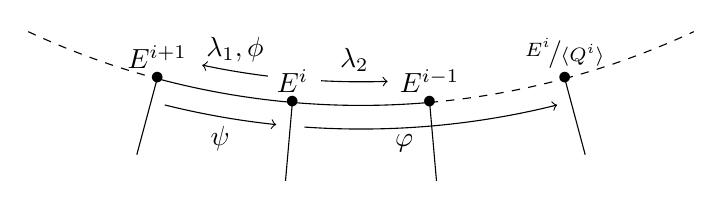
\begin{tikzpicture}[scale=1]
\coordinate (A) at (245:10);
\coordinate (B) at (255:10);
\coordinate (B') at (255:11);
\coordinate (B1) at (256:10.3);
\coordinate (C) at (265:10);
\coordinate (C') at (265:11);
\coordinate (D) at (275:10);
\coordinate (D') at (275:11);
\coordinate (E) at (285:10);
\coordinate (E') at (285:11);
\coordinate (F) at (295:10);
\coordinate (F') at (295:11);
\coordinate (G) at (305:10);
\coordinate (B2) at (258:9.7);
\coordinate (C1) at (266:10.3);
\coordinate (C2) at (267:9.7);
\coordinate (encre) at (273:10.5);
\draw (A) arc(245:255:10)[dashed];
\draw (B) arc(255:275:10);
\draw (D) arc(275:285:10)[dashed];
\draw (E) arc(285:295:10)[dashed];
\draw (B) node[above] {$E^{i+1}$} node{$\bullet$};
\draw (C) node[above] {$E^{i}$} node{$\bullet$};
\draw (D) node[above] {$E^{i-1}$} node{$\bullet$};
\draw (E) node[above] {$\nicefrac{E^i}{\langle Q^i \rangle }$} node{$\bullet$};
\draw (encre) node {$\varphi$};
\draw (B)--(B');
\draw (C)--(C');
\draw (D)--(D');
\draw (E)--(E');
\draw (B1) arc(256:264:10.3) [->] node[below,midway] {$\psi$}; %flèche représentant \psi
\draw (B2) arc(258:263:9.7) [<-] node[above,midway] {$\lambda_1, \phi$}; %flèche représentant 
\draw (C2) arc(267:272:9.7) [->] node[above,midway] {$\lambda_2$}; %flèche représentant 
\draw (C1) arc(266:284:10.3) [->];% node[below,midway,fill=white] {$\varphi $};

%\draw (260:10.75) node{}
%\draw (0,0) arc (245:255:10)[dashed] node[above] {$C$} node{$\bullet$} --(0:1.5);
%\draw (0,0) arc (245:255:10)[dashed] arc (255:265:10) node[above] {$E^i$} node{$\bullet$} --(0:1.5);
%\draw (-1,0) arc (245:255:10) node[above] {$C2$} node{$\bullet$} --(90:1)[color=yellow];
%\draw (-1,0) arc (245:255:10) node[above] {$C$} node{$\bullet$} --(310:1.5)[color=red];
%\draw (0,0) arc (245:255:10)[color=white] node[above] {$C$} node{$\bullet$} arc (255:265:10) node[above] {$E^i$} node{$\bullet$} arc (265:275:10) node[above] {$E$} node{$\bullet$} arc (275:285:10) node[above] {$F$} node{$\bullet$} arc (285:295:10) node[above] {$G$} node{$\bullet$} ; 
\end{tikzpicture}
\end{center}
\caption{ Example for the case $\ell=2$ } 
\end{figure}

\begin{proof}
We will first prove that the isogeny $E^{i+1} \rightarrow \nicefrac{E^{i+1}}{\phi(R)}$ is horizontal and associated to $\lambda_2$.
\newline
Since $\ell^j\phi(R)=\phi(\ell^{j-1}Q^i)$ and $Q^i$ is associated to $\lambda_2$ then the $\ell$-isogeny $\psi$ with kernel $\ell^{j}\phi(R)$ is the dual isogeny of $\phi$ because it is the one who anhiliates the $\ell$-torsion (here $\langle P, \ell^{j-1}Q^i \rangle$) together with $\phi$ on $E^i$. Thus we have proved that $\psi$ is associated to $\lambda_2$ and horizontal. 
\newline
Since we have $\psi(\phi(R))=Q^i$, this tells us that the isogeny $\Upsilon$ with kernel $\phi(R)$ is the composition of $\psi$ with the isogeny $\varphi$ of kernel $\langle Q^i \rangle$. Thus the isogeny $\Upsilon$ is horizontal of degree $\ell^{j+1}$ and associated to $\lambda_2$.
\newline
Let $W$ a point of order $\ell^{h+j+1}$ such that $\ell^hW=\phi(R)$, let $T$ a point such that $\phi(T)=W$. From $\ell^h\phi(T)=\phi(R)$ we deduce that $\ell^{h+1}T=Q^i$ and that $T$ is of order $\ell^{j+h+1}$. Let denote $\widehat{\phi}$ the dual isogeny of $\phi$, since $W$ is a division point of $\phi(Q^i)$, $\widehat{\phi}$ is the $\ell$ isogeny generated by $\ell^{h+j}W=\ell^j\phi(R)=\ell^{j-1}\phi(Q)$. As $\ell^{h}\widehat{\phi(W)}=\ell^h\widehat{\phi}(\phi(T))=\ell^{h+1}T=Q^i$, thus by hypothesis we have $\pi(\widehat{\phi}(W))=\lambda_2\widehat{\phi}(W)$. Moreover we have $\widehat{\phi} (\phi(T))=\widehat{\phi}(W)$ this implies that $\pi(\ell T)=\pi(\widehat{\phi}(W))=\lambda_2\widehat{\phi}(W)=\lambda_2(\ell T)$. Thus we have for $T$: $\pi(T)=\lambda_2 T + P$ with a $\ell$ torsion point $P$ associated to the "eigenspace" of $\lambda_1$. Then with the action of $\phi$ associated to $\lambda_1$ we have $\pi(\phi(T))=\pi(W)=\lambda_2\phi(T)=\lambda_2W$. 
\end{proof}

\begin{prop}
Let $Q$ be a point of $\ell^j$ torsion with $j>0$ then there exists a division point $R$ of $Q$ of order $\ell^{h+j}$ with $\pi(R)=\lambda_2R$ if and only if the $\ell^j$ isogeny with kernel $\langle Q \rangle $ is horizontal.
\end{prop}

\begin{proof}
In \ref{propcentrale}, the $\Leftarrow$ has been proved. Now we will prove the other way.
\newline
We do a recursive proof. The initial step is the conjecture \ref{conjecture}.
\newline
Recursive step: we consider that the property is true to the rank $j>1$, then we will have to prove it for $j+1$.
We consider then $S$ a point of order $\ell^{j+1}$ with $T$ a division point of $S$ of order $\ell^{h+1+j}$ with $\pi(T)=\lambda_2T$.We know that the $\ell^j$ isogeny $\phi$ generated by $\langle \ell S \rangle$ is horizontal and associated to $\lambda_2$. We then have $\phi(S)$ a point of order $\ell$ and $\phi(T)$ a point of order $\ell^{h+1}$ with $\pi(\phi(T))=\lambda_2\phi(T)$. Thus by applying the conjecture \ref{conjecture} we have the isogeny $\psi$ with kernel $\langle \phi(S) \rangle$ horizontal, therefore the isogeny with kernel $\langle S \rangle$ who is equal to the composition of $\psi$ with $\phi$ is horizontal.
\end{proof}

\begin{prop}
For $\phi$: $E \rightarrow E'$ a $r$-isogeny  with $r \wedge \ell=1$ an odd prime, and $P$ a $\ell^i$ primitive torsion point, with $i>0$ such that $E \rightarrow E / \langle P \rangle $ is horizontal and $P$ is associated to $\lambda_1$. Then the isogeny  $E' \rightarrow E' / \langle \phi(P) \rangle$ is also horizontal.
\end{prop}

\begin{proof}
We just have to prove that there exists a $\ell^{h+i}$ primitive torsion point $V$ dividing $\phi(P)$ such that $\pi(V)=\lambda_1P$.
Since $P$ is a point that generates a horizontal isogeny then there exists a point $R$ of order $\ell^{h+i}$ dividing $P$. Since $\phi$ is a $r$ isogeny then $\phi$ doesn't change the order of $P$ and $R$, moreover the frobenius commutes with $\phi$ (because this one is defined on $\mathbb{F}_q$) then we have $\pi(\phi(R))=\lambda_1\phi(R)$ which proves the assertion.
\end{proof}

We have thus proved that the image of a $\ell$ horizontal basis by an $r$ isogeny with $r \wedge \ell = 1$ is still an $\ell$ horizontal basis. Now we will show how to extend this result for curves not on the crater.


\begin{defi}
Let $\ell$ an integer we denote by
$C(\ell)=\{\left(\begin{array}{cc}
a & b\\
0 & d
\end{array}\right): ad= \ell, a>0,0\leqslant b <d, gcd(a,b,d)=1\}$
\end{defi}

\begin{lem}
Let consider $E$ an elliptic curve defined on $\mathbb{C}$ such that $E$ is not at the crater of the volcano of $\ell$-isogeny. We consider the $\mathbb{Z}$ lattice associated (up to isomorphism) to $E:[1,\tau]$. The ascending $\ell$-isogeny is the one associated to $M=\left(\begin{array}{cc}
\ell & 0\\
0 & 1
\end{array}\right)$ with $M \in C(\ell)$
\end{lem}

\begin{proof}
Let consider $E_1$ on $\mathbb{C}$, we denote by $[1,\tau_1]$ the lattice associated to $E_1$. For $\sigma \in C(\ell)$, $d[1,\sigma \tau_1]$ is the lattice associated to an $\ell$ isogenous curve of $E_1$ (see Theorem 11.23 and Lemma 11.24 \cite{Cox89}).
\newline
We consider a $\mathbb{Z}$-basis of the endomorphism ring $[1,\omega_1]$ associated to the elliptic curve $[1,\tau_1]$ since we are not on the crater of the volcano we know that $\ell | \omega_1$. 
\newline
Let's consider $\ell$-isogenous curves of $E_1$, they are associated to lattices $\ell[1,\frac{\tau_1+k}{\ell}]$ with $k \in [0..\ell-1]$ and the lattice $[1,\ell \tau_1]$. Now we consider $\alpha \in End([1,\tau_1])$ such that $f\mathcal{O}_K=\mathbb{Z}[\alpha]$ we can express $\alpha = a + b \tau_1$ with $a,b \in \mathbb{Z}, a \wedge b =1$. From the work of Kohel \cite{Kohel96} we know that $\alpha$ will be included in only one of the $\ell$ isogenous curve. 
\begin{enumerate}
\item $\alpha \in \textsf{End}(\ell[1,\frac{\tau_1+k}{\ell}]) $ is equivalent to $\ell | (a-kb)$,
\item $\alpha \in End([1,\ell\tau_1]) $ is equivalent to $\ell | b$.
\end{enumerate}
 Thus if we have $\alpha $ who belongs to two different sets of ${ End(\ell[1,\frac{\tau_1+k}{\ell}]), k \in [0..\ell-1] \bigcup End([1,\ell\tau_1])}$ then it should belong to all of them. However we know that $\alpha = \ell \alpha'$ since we are not on the crater of the volcano thus the imaginary part of $\alpha$ is divisible by $\ell$ thus $b$ is divisible by $\ell$. 
\newline 
Since we obtain $[1,\ell \tau_1]$ by acting with the matrix $C(\ell,0,1)=\left(\begin{array}{cc}
\ell & 0\\
0 & 1
\end{array}\right)$ we can conclude.
\end{proof}

\begin{prop}
Let consider $E_1$ and $E_2$ two elliptic curve $r$-isogenous not on the crater of $\ell$ isogeny volcano with $r$ prime different from $\ell$, we denote by $E_{1c}$ (resp. $E_{2c}$) the elliptic on the crater of the $\ell$ isogeny volcano of $E_1$ (resp. $E_2$) obtained by a composition of only $\ell$ ascending isogeny. Then $E_{1c}$ and $E_{2c}$ are also $r$-isogenous.
\end{prop}

\begin{proof}
We first consider $E_{1u}$ and $E_{2u}$ curves which are $\ell$ isogenous to $E_1$ and $E_2$ and $1$ level above in the volcano, we prove then that $E_{1u}$ and $E_{2u}$ are also $r$ isogenous.
\newline
Let consider $\tau_1$ (resp. $\tau_2$)  such that $[1,\tau_1]$ (resp. $d[1,\tau_2]$) is associated to $E_1$ (resp. $E_2$), with $\tau_2$ such that $\tau_2=\frac{a\tau_1+b}{d}$ and $\left(\begin{array}{cc}
a & b\\
0 & d
\end{array}\right)$ in $C(r)$. 
\newline
We denote $C(\ell,0,1)= \left(\begin{array}{cc}
\ell & 0\\
0 & 1
\end{array}\right) \in C(\ell)$
\newline
By the previous lemma we have the curve $E_{1u}$ associated to $[1,C(\ell,0,1)\tau_1]$ and the curve $E_{2u}$ associated to $d[1,C(\ell,0,1)\tau_2]$.
We want to prove that there exists $\sigma' \in C(r)$ such that $C(\ell,0,1)\tau_2=\sigma' C(\ell,0,1)\tau_1$, thus by Theorem 11.23 and Lemma 11.24 of \cite{Cox89} we can then conclude that the curve $E_{1u}$ associated to $[1,C(\ell,0,1)\tau_1]$ is $r$ isogenous to the curve $E_{2u}$ associated to $d[1,C(\ell,0,1)\tau_2]$.
\newline
We have $C(\ell,0,1)\tau_2=\frac{\ell a\tau_1+\ell b}{d}$, since $\forall k \in \mathbb{N}$ $[1,\frac{\ell a\tau_1+\ell b}{d}]=[1,\frac{\ell a\tau_1+\ell b-kd}{d}]$ we can consider that we have $0 \leqslant \ell b<d$.
Let's consider $\sigma' \in C(r)$ then we have $\sigma'(\ell \tau_1)=\frac{a'\ell \tau_1+ b'}{d'}$ thus to have $\frac{a'\ell \tau_1+ b'}{d'}=\frac{\ell a\tau_1+\ell b}{d}$ we take $a'=a, b'=\ell b, d'=d$ wich defines us $\sigma' \in C(r)$. We can recap this proof in the following commutative diagram :
\begin{center}
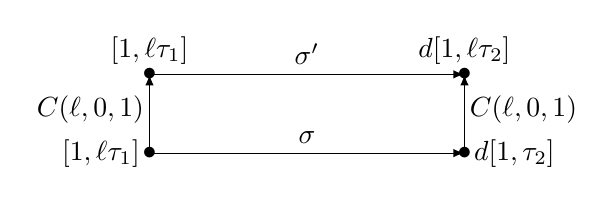
\begin{tikzpicture}[scale=0.5]
\coordinate (C) at (0,0);
\coordinate (D) at (8,0);
\coordinate (A) at (0,2);
\coordinate (B) at (8,2);
\coordinate (E) at (-1.5,0.5);
\coordinate (F) at (9.5,0.5);
\draw (A) node[above] {$[1,\ell\tau_1]$} node{$\bullet$};
\draw (B) node[above] {$d[1,\ell\tau_2]$} node{$\bullet$};
\draw (C) node[above,left] {$[1,\ell\tau_1]$} node{$\bullet$};
\draw (D) node[above,right] {$d[1,\tau_2]$} node{$\bullet$};
\draw (E) node[above] {$C(\ell,0,1)$};
\draw (F) node[above] {$C(\ell,0,1)$} ;
\draw (A)--(B) [>=latex,->] node[above,midway] {$\sigma'$};
\draw (C)--(D)[>=latex,->] node[above,midway] {$\sigma$};
\draw (C)--(A)[>=latex,->] ;
\draw (D)--(B)[>=latex,->] ;
\end{tikzpicture}
\end{center}

 We can then conclude recursively to obtain the result for curves on the crater.
\end{proof}

\section{Interpolating the two bases}

\bibliographystyle{plain}
\bibliography{refs}

\end{document}
